\section{Implementierung der Holdback Queue}

Wie bereits in Kapitel \ref{Problemstellungen} erläutert, wird die Holdback Queue mit zwei verschiedenen Strukturen implementiert.

Für die Struktur des HeapSorts gilt, dass jedes Element die Form \{$[$Nnr, Msg, TSclientout, TShbqin$]$, Höhe, linkerTeilbaum, rechterTeilbaum\} hat. Außerdem ist die Nnr des Wurzelelements stets kleiner als die der Kinderelemente. Die beiden Kinderelemente werden nicht miteinander verglichen. Diese Form des Heaps nennt sich Min Heap (siehe Abb. \ref{fig:binHeap}).

\begin{figure}[htbp]
\begin{center}
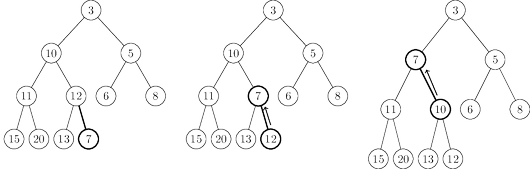
\includegraphics[scale=0.7]{Latex/Bilder/heapExample.png}
\caption[Binary Min Heap Insert]{Binary Min Heap Insert\footnotemark}\label{fig:binHeap} 
\end{center}
\end{figure}
\footnotetext{\url{https://rosalind.info/glossary/algo-binary-heap/}}

Für das Entfernen eines neuen Elements entsteht dadurch der Vorteil, dass das Element im Normalfall die Wurzel des Heaps ist, da es die kleinste Nachrichtennummer haben sollte und somit ganz oben als Wurzel gespeichert ist. Auch beim Einfügen des Elements ist der Heap von Vorteil, da die Elemente ohne erkennbare Sortierung (siehe Abbildung \ref{fig:HBQFilesEntry}) vom Server in den Heap eingefügt werden. Die Elemente werden am höchsten freien Index eingefügt und wandern dann im Heap nach oben, bis sie ihre Position erreicht haben. Im Beispiel ist zu sehen, wie das Element mit der Nummer 7 eingefügt wird und solange mit dem Elternknoten getauscht wird, bis dieses größer ist. 

Da das Konzept des HeapSort Algorithmus darauf aufbaut, dass die neuen Elemente als Blatt eingefügt und die sortierten Elemente als Wurzel entfernt werden, kann der implementierte Heap aus dem Praktikum 2 nur teilweise wiederverwendet werden. Da dieser ein Max Heap ist, das heißt das größte Element ist die Wurzel, jetzt aber ein Min Heap benötigt wird, wird der Code größtenteils wiederverwendet, aber in Teilen angepasst.
Der Max Heap wurde zusammen mit Leon Schwarzenberger entwickelt und implementiert. Für weitere Informationen und Entwürfe über die einzelnen Heap Funktionen siehe Anhang \ref{anhang} oder \cite{sortAlgo}.

\begin{figure}[htbp]
\begin{center}
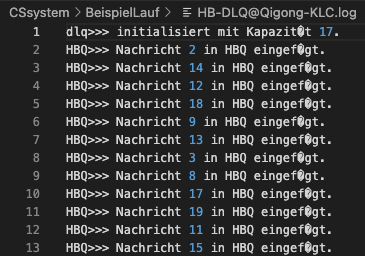
\includegraphics[scale=0.6]{Bilder/HBQFilesEntry.png}
\caption{\label{fig:HBQFilesEntry} Nachrichtendienst \cite{HBQlogging}} 
\end{center}
\end{figure}

\subsection{Operationen}

\subsubsection{initHBQ}

Beim Initialisieren der Holdback Queue liegt das größte Problem darin, die Queue auf einem Node zu speichern. Das ermöglicht die Erlang Funktion spawn/1, welcher als Parameter die Funktion übergeben wird, welche gestartet werden soll. Hierbei wird ein neuer Prozess erzeugt und initialisiert. Die ProzessID dieses neu erzeugten Prozesses wird als Rückgabewert zurückgegeben und in einer Variable gespeichert. 
Die globale Registrierung des Prozesses findet über den Aufruf register/2 statt. Als Parameter werden hier einmal die ProzessID des zu registrierenden Prozesses übergeben und das Atom unter welchem dieser Prozess gespeichert werden soll. 
Außerdem wird die Initialisierung der Delivery Queue über die Holdback Queue aufgerufen. Diesem Aufruf wird der Parameter DLQ-Limit, also die maximale Größe der Delivery Queue, mit übergeben. 

Durch Rekursion kann der Status des Prozesses, also in diesem Falle unter anderem die Informationen über die Holdback und Delivery Queue, vollständig in den Parametern der Funktion gehalten werden (frei nach \cite{learnErlang}). Der Prozess der Holdback Queue wird hierfür über die Funktion loop gestartet. Dieser Funktion wird als Parameter die Holdback Queue, dessen nächster freier Index oder dessen Größe, die Delivery Queue, dessen maximale Größe und die logging Datei übergeben. Somit können diese über jeden loop Aufruf beschrieben und gelesen werden. 
Ob der nächste freie Index oder die aktuelle Größe übergeben wird, hängt von der Struktur der Holdback Queue ab. 

\subsubsection{checkHBQ} \label{checkHBQ}

Da die Nachrichten der Holdback Queue regelmäßig auf Auslieferbarkeit geprüft werden sollen, wurde hierfür eine weitere Funktion implementiert. 
In dieser wird das derzeitige erste Element der Holdback Queue (im Folgenden 'SmallestElem')  mit der von der Delivery Queue erwarteten Nummer ('ExpNrDLQ') verglichen. 
Somit kann erkannt werden, ob Elemente aus der Holdback Queue verworfen oder an die Delivery Queue ausgeliefert werden sollen. 
Wenn zum Beispiel SmallestElem == ExpNrDLQ gilt, dann wird SmallestElem an die Delivery Queue ausgeliefert. Im Falle SmallestElem $<$ ExpNrDLQ wird das SmallestElem verworfen, da es nicht mehr benötigt wird und ansonsten die Holdback Queue nur blockieren würde. Benötigt wird es nicht mehr, da die Delivery Queue als aufsteigende Liste ohne Duplikate und ohne fehlende Nachrichtennummern definiert ist. Alle Nachrichten, welche eine kleinere Nachrichtennummer als das aktuell kleinste Element der Delivery Queue haben, werden von dieser nicht mehr angefragt und können somit aus der Holdback Queue verworfen werden.  
Für den Fall, dass die Holdback Queue keine Elemente mehr enthält wird eine entsprechende Ausgabe geloggt. 

\begin{figure}[htbp]
\begin{center}
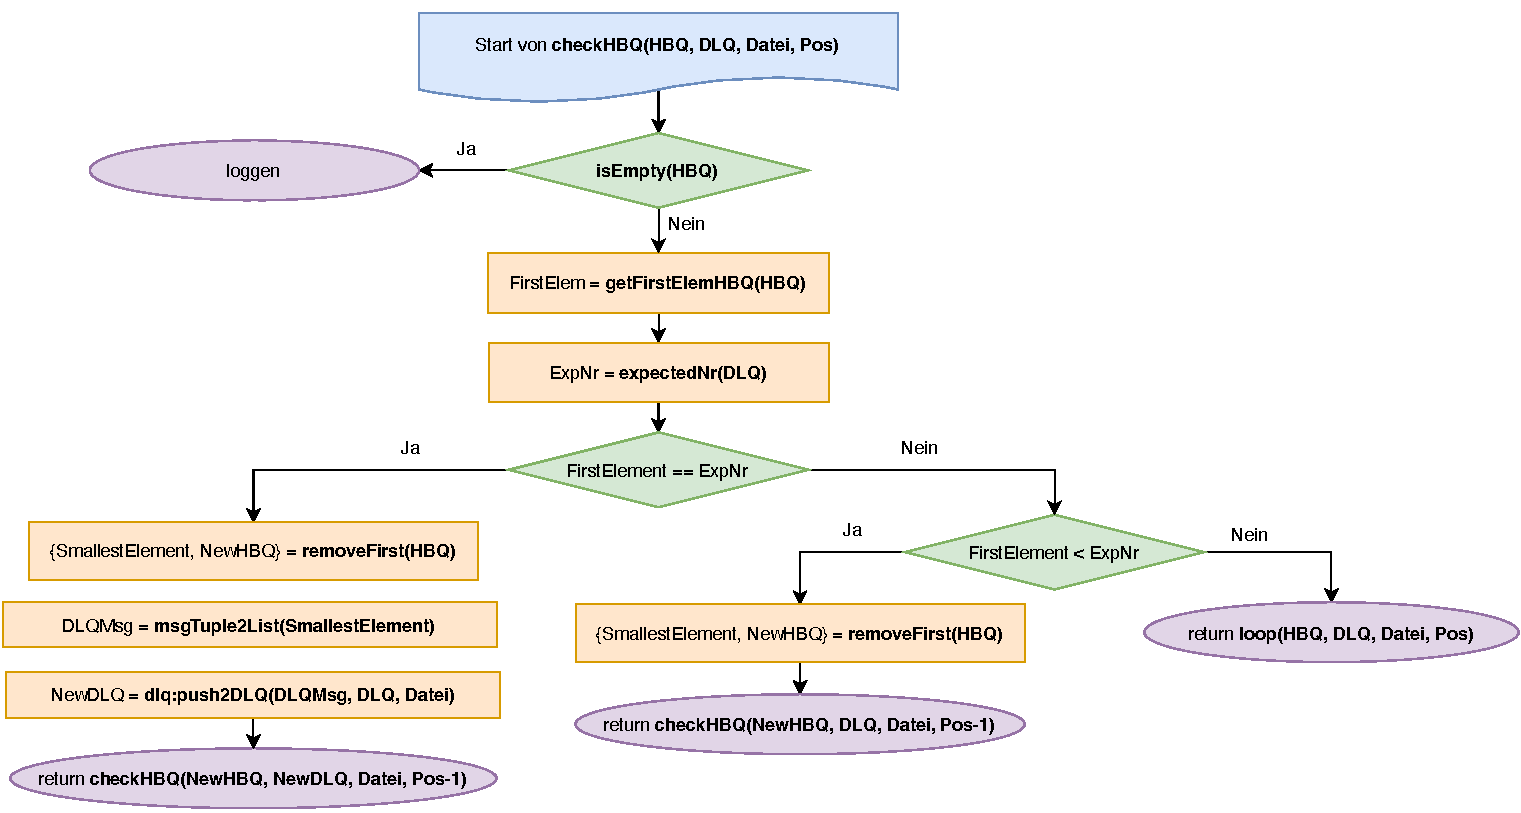
\includegraphics[scale=0.58]{Latex/Bilder/checkHBQ.pdf}
\caption{checkHBQ}\label{fig:checkHBQ}
\end{center}
\end{figure}

Wenn also zum Beispiel am Anfang nur Elemente $>$ 3 in die Holdback Queue eingefügt wurden, dann fehlen die Elemente 1, 2 und 3 zum Einfügen in die Delivery Queue. In der Fehlermeldung steht folglich "Fehlernachricht für Nachrichten 1 bis 3 generiert.". Die 3 wird als Nachricht zusätzlich in die Delivery Queue eingefügt.

Die Funktion wird nach jeder Ausführung der pushHBQ Funktion aufgerufen. Somit ist sichergestellt, dass nach jeder Veränderung der Queue einmal geprüft wird, ob diese noch synchronisiert ist und keine für die Delivery Queue geeignete Nachricht vom Server geschickt wurde.

\subsubsection{pushHBQ} 

In dieser Funktion wird eine Nachricht in die Queue geschrieben. Die Nachricht enthält die entsprechende Nachrichtennummer, den Inhalt der Nachricht und einen Timestamp, wann der Client die Nachricht abgeschickt, bzw. die Holdback Queue diese empfangen hat. Wie bereits beschrieben wird bedingt durch die fehlende Sortierung der Clients jedes Element als Blatt eingefügt.
 
Zum Bestimmen des Pfades der nächsten freien Blatts wird wie in der letzten Praktikumsaufgabe die sortv.erl Datei \cite{sortv} verwendet. Hier wird als Parameter die Position, also der höchste freie Index mit übergeben. Dieser muss also bei jedem Einfügen eines Elements erhöht und beim Löschen eines Elements um eins verkleinert werden. 

\begin{figure}[htbp]
\begin{center}
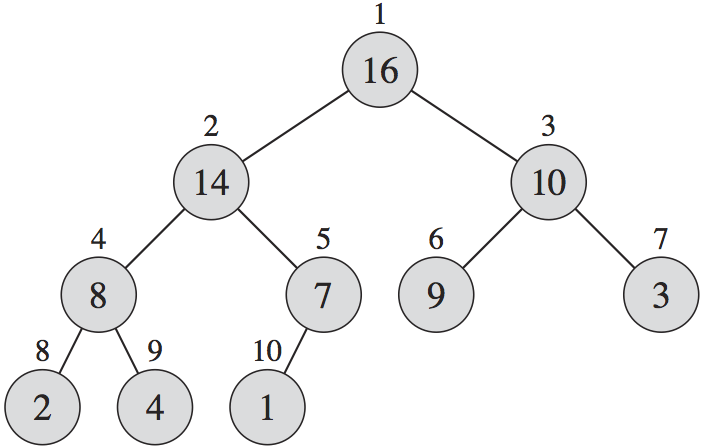
\includegraphics[scale=1]{Latex/Bilder/heapIndex.png}
\caption[Binary Heap Index]{Binary Heap Index\footnotemark}\label{fig:binHeapIndex}
\end{center}
\end{figure}
\footnotetext{\url{https://weibeld.net/algorithms/data-structures.html}}

\begin{lstlisting}
% sortv.erl
% @author: Prof Dr Christoph Klauck, HAW Hamburg 
calcPath(Number) -> calcPath(Number,[]).
% aktuelle Position ist Wurzel
calcPath(1,Accu) -> Accu;
% aktuelle Position ist gerade
calcPath(Number,Accu) when Number rem 2 =:= 0 -> calcPath(Number div 2,[l|Accu]);
% aktuelle Position ist ungerade
calcPath(Number,Accu) when Number rem 2 =/= 0 -> calcPath((Number-1) div 2,[r|Accu]).	
\end{lstlisting}

Anhand dieses Indexes kann der Pfad durch modulo Rechnungen bestimmt werden. Wird wie im Beispiel in der Abbildung \ref{fig:binHeapIndex} eine ungerade Position, in diesem Fall die 11, übergeben, wird der Pfad $[l|r|r]$ zurückgegeben. Es müssen also zuerst der linke Teilbaum und dann zweimal der rechte Teilbaum gewählt werden, um in das nächste freie Blatt zu gelangen.
Die Position des höchsten Index wird als Integer zusammen mit der Holdback Queue als Parameter in der loop Funktion mit übergeben und somit rekursiv gespeichert. 

Da in der Delivery Queue nur eine bestimmte Anzahl an Nachrichten stehen kann, wird bei der Holdback Queue ab einer erreichten Größe von $\frac{2}{3}*sizeOf(DLQ)$ der Inhalt der Queue reduziert. Dafür wird geprüft, wie groß die Lücke zwischen den beiden Queue ist. Ein Beispiel dafür ist in Abbildung \ref{fig:BeispielHBQFehler} zu sehen. Hier hat die Holdback Queue diese bestimmte Größe erreicht und die Lücke in der Delivery Queue wird dementsprechend aufgefüllt. Aufgefüllt werden hierbei allerdings nicht alle fehlenden Nachrichten, sondern nur die von der Delivery Queue zuletzt erwartete. Eine ähnliche Fehlermeldung wie in der Abbildung wird in Textform in diese Nachricht als Msg eingetragen. 

\begin{figure}[htbp]
\begin{center}
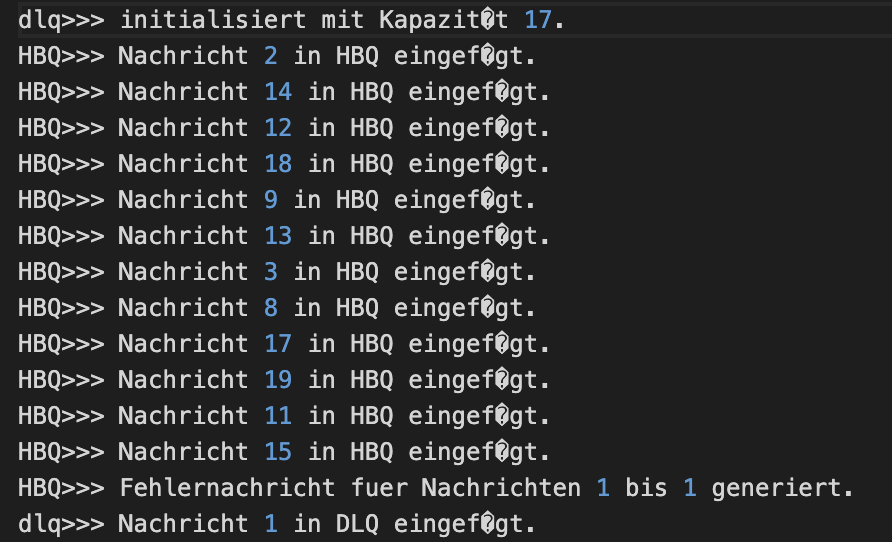
\includegraphics[scale=0.6]{Bilder/BeispielHBQFehler}
\caption{\label{fig:BeispielHBQFehler} Fehlermeldung Beispiel \cite{HBQfehler}} 
\end{center}
\end{figure}

Die Elemente welche aus der Holdback Queue an die Delivery Queue gesendet wurden, müssen aus der Holdback Queue gelöscht werden, da ansonsten die Größe der Queue nicht aktualisiert werden kann. 
Dies geschieht durch regelmäßige Kontrolle nach dem Einfügen eines Elements, ob das kleinste Elemente der Holdback Queue in die Delivery Queue eingefügt werden kann (siehe \ref{checkHBQ}).
Das kleinste Element der Holdback Queue ist dessen Wurzelelement. Dieses muss größer gleich der erwarteten Nummer der Delivery Queue sein. 
Ansonsten kommt es zu einem Ausnahmefall, welcher aber bedingt durch das Verwerfen von Nachrichten, welche kleiner als die erwartete Nummer sind, eigentlich nicht vorkommen dürfte. 

Ein weiteres Problem entsteht, wenn Elemente eingefügt werden, welche eine kleinere Nachrichtennummer haben als das zu erwartende nächste Element der Delivery Queue. In diesem Falle wird die einzufügenden Nachricht verworfen und es wird NNr<expNrDLQ an den Prozess gesendet, welcher die Holdback Queue beauftragt hat.

\subsubsection{deliverMSG}

In dieser Funktion wird die Delivery Queue über die Holdback Queue beauftragt die zu der übergebenen Nachrichtennummer zugehörige Nachricht zu senden. Der Client welcher die Nachricht empfangen soll wird als ProzessID mit im Parameter der Funktion übergeben. 
Über den Funktionsaufruf dlq:deliverMSG(MSGNr, ClientPID, Queue, Datei) wird also die entsprechend zu sendende Nachrichtennummer, die ProzessID, die Delivery Queue und die in die zu loggende Datei übergeben. 
Wenn die übergebene Nachricht nicht verfügbar ist, dann wird die Nachricht mit der nächst größeren Nummer gesendet. 
Als Antwort von dem Prozess der Holdback Queue wird dann die gesendete Nachrichtennummer gesendet. 

\subsubsection{listADT}

Diese Funktion ist aufgeteilt in zwei verschiedene Funktionen: listHBQ und listDLQ. 
Es wird in beiden der Inhalt der jeweiligen Queue ausgegeben. Dabei wird die Reihenfolge der Queue beibehalten. Ausgegeben werden alle enthaltenden Nachrichtennummern in Form einer Liste. 

\paragraph{listHBQ}
Für diese Funktion wird über alle Elemente der Holdback Queue iteriert und jeweils die Nachrichtennummer in eine separate Liste geschrieben werden. 
Da die Holdback Queue hier in einer Heap Struktur umgesetzt ist, gibt es zwei mögliche Sortierungen. Zum einen könnte nach Index sortiert werden. Dementsprechend würde das Wurzelelement als erstes ausgegeben werden, dann alle Elemente mit der nächst kleinsten Höhe von links nach rechts gelesen usw..
Die andere Möglichkeit wäre es den Heap bei der Ausgabe zu sortieren. Es würde also das Wurzelelement als erstes ausgegeben werden, vor der nächsten Ausgabe wird dann aber erst der Heap neu strukturiert. Das Element mit dem höchsten Index wird die neue Wurzel. Dann versickert dieses so lange nach unten, bis es keinen kleineren Teilbaum mehr hat. Erst danach wird das nächste Element (also wieder die Wurzel) ausgegeben. 
Der Vorteil der Index-Sortierung ist die kleinere Laufzeit, da im Vergleich zur Nachrichtennummer-Sortierung nicht nach jeder Ausgabe neu strukturiert werden muss. Allerdings sind bei der Index-Sortierung die Nachrichtennummern in der Ausgabe zufällig, was z.B. das händische Finden eines Elements aufwändiger machen würde. 
Da die Funktionalität in diesem Falle im Vordergrund steht, wird bei listHBQ eine Liste in aufsteigend sortierter Reihenfolge ausgegeben. 

Die Ergebnisse werden in eine log Datei geschrieben und bei Erfolg wird als Rückgabewert ein ok als Antwort gesendet.

\paragraph{listDLQ}
Da es schon eine Funktion listDLQ für die Delivery Queue gibt, wird diese hier verwendet. 
Als Queue wird einfach die in der Holdback Queue gespeicherte DLQ übergeben und die zurückgegebene Liste wird dann in die Logging Datei geschrieben. 

\subsubsection{dellHBQ}

Um die HBQ zu löschen muss durch die rekursive Implementierung die Funktion loop/4 beendet werden. Dadurch, dass diese Funktion als Schleife implementiert ist, wird durch den dellHBQ die Abbruchbedingung simuliert. Nach diesem Aufruf sind dann weder die Elemente innerhalb der Queue noch vorhanden, noch ist die PID der Queue weiterhin referenziert. 
Außerdem wird das Löschen der Delivery Queue von dieser Funktion initialisiert. 

